\chapter{Technical system overview}

\section{Function requirements}
This section specifies the requirements set for the functions mentioned in figure \ref{fig:funcarch}.
\subsection{Generate flow}
In the project plan, a literature overview is given on perfusion phantoms, for a variety of organs, but also on physiological factors: perfusion rates, blood pressures, rates of stenosis et cetera. The TFR-GF requirements are based on the estimates by \cite{uren1994relation}, summarised in appendix \ref{app:physoverview}, \cite{chiribiri2013normal}, \cite{ho2014dynamic}, summarised in appendix \ref{app:physoverview_ho}, and \cite{slart2015pres}.

Decisions and design choices are given in table \ref{tab:genflow_text}, quantitative requirements are given in table \ref{tab:genflow_quan}.

\begin{table}[H]
\caption{Textual requirements for function: Generate flow}
\label{tab:genflow_text}
\begin{tabular}{p{25mm}|p{115mm}|}
	\textbf{Requirement number} & \multicolumn{1}{c}{\textbf{Description}} \\
	\hline
	TFR-GFT01 & A constant flow is to be generated, i.e. non-pulsatile. \\
	TFR-GFT02 & Flow generators need to be interchangeable. \\
	TFR-GFT03 & Flow feedback control for flow generators. \\
	\cline{2-2}
\end{tabular}
\end{table}

\textbf{TFR-GFT01} is based on reducing the complexity of the set-up. The ROI based AIF averages the intensity over time, which removes the pulsatile nature. Furthermore, the heart rate cannot be determine in the measurements results. Therefore, pulsatile flow is not a priority.
\textbf{
TFR-GFT02} is based on maintaining flexibility such that the most optimal flow generator can be chosen based on the requirements for a specific experiment.

\textbf{TFR-GFT03} is based on ensuring reliability; no validation can be performed when the flow is not controlled.

\begin{table}[H]
\caption{Quantitative requirements for function: Generate flow}
\label{tab:genflow_quan}
\begin{tabular}{p{24mm}|p{65mm}ccp{21mm}|}
	\textbf{Requirement number} & \multicolumn{1}{c}{\textbf{Description}} & \multicolumn{1}{c}{ } & \multicolumn{1}{c}{\textbf{Value}} & \multicolumn{1}{c}{\textbf{Unit}} \\
	\hline
	TFR-GFQ01*	& Upper limit myocardial perfusion. 		 		& = 				& 300 				&  mL/min/100g \\
	TFR-GFQ02* 	& Lower limit myocardial perfusion. 				& = 				& 60 				& mL/min/100g \\
	TFR-GFQ03* 	& Typical perfusion rate during stress. 	 		& > \spacing < 		& 190 \spacing 300 	& mL/min/100g \\
	TFR-GFQ04*  	& Typical perfusion rate during rest. 			& > \spacing < 		& 60 \spacing 95 	& mL/min/100g \\
	TFR-GFQ05**	& Upper limit cardiac output.				 		& =					& 8 				& L/min \\
	TFR-GFQ06+		& Lower limit arterial pressure.				& =					& 56				& mmHg \\
	TFR-GFQ07+		& Upper limit arterial pressure.				& = 				& 155				& mmHg \\
	TFR-GFQ08		& Mean Arterial Pressure (MAP)\footnotemark. 	& = 				& 89				& mmHg \\
	TFR-GFQ09		& Typical MAP.								 	& > \spacing <		& \invchar 70 \spacing 110	& mmHg \\
	TFR-GFQ10 	& Feedback control accuracy 						& =					& 5					& \% \\
	\cline{2-5}
\end{tabular} \\
\raggedright
\textit{* combined flow to myocardium, indicated by blue arrows in figure \ref{fig:sim_heart}.} \\
\textit{** flow \textbf{not} entering the myocardium, indicated by red arrow in figure \ref{fig:sim_heart}.} \\
\textit{+ based on diastolic and systolic blood pressures, respectively. Measured at dashed line P in figure \ref{fig:sim_heart}.}
\end{table}

\footnotetext{Calculated as: $MAP \simeq DP + \sfrac{1}{3} (SP-DP)$}

\begin{figure}
\centering
\begin{minipage}{.5\textwidth}
  \centering
  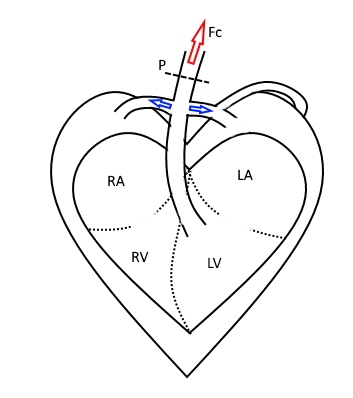
\includegraphics[width=0.7\linewidth]{./images/simplified_heart.png}
  \captionof{figure}{Simplified, schematic overview of the heart.}
  \label{fig:sim_heart}
\end{minipage}%
\begin{minipage}{.5\textwidth}
  \centering
  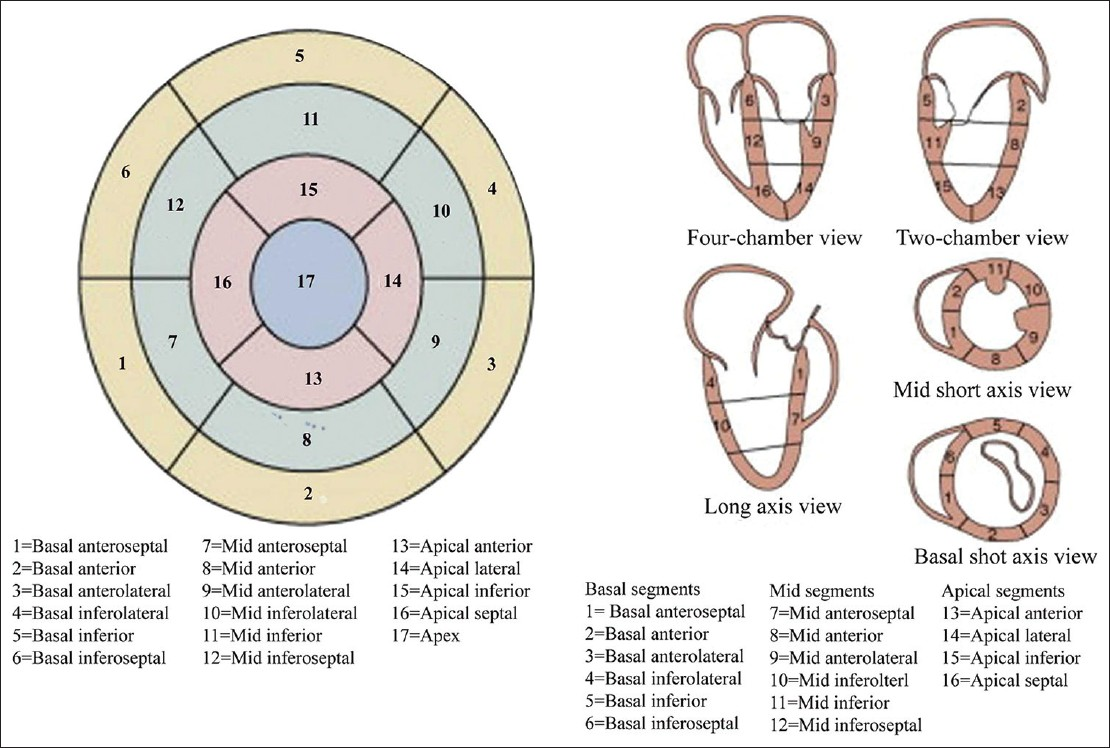
\includegraphics[width=0.95\linewidth]{./images/17_segment.jpg}
  \captionof{figure}{17-segment heart model}
  \label{fig:segment_heart}
\end{minipage}
\end{figure}

\subsection{Measuring flow and pressure}
\begin{table}[H]
\caption{Quantitative requirements for function: Measure flow and pressure}
\label{tab:measflow_quan}
\begin{tabular}{p{25mm}|p{65mm}ccp{20mm}|}
	\textbf{Requirement number} & \multicolumn{1}{c}{\textbf{Description}} & \multicolumn{1}{c}{ } & \multicolumn{1}{c}{\textbf{Value}} & \multicolumn{1}{c}{\textbf{Unit}} \\
	\hline
	TFR-MFPQ01	& Flow measuring accuracy. 		 			 & <= 		& 5 		& \% \\
	TFR-MFPQ02 	& Pressure measuring accuracy.		 		 & <= 		& 5 		& \% \\
	TFR-MFPQ03 	& Absolute flow resolution.				 	 & >=	 	& 1 		& mL/min \\
	TFR-MFPQ04  & Sampling rate.					 		 & >= 		& 10 		& Hz \\
	\cline{2-5}
\end{tabular} \\
\raggedright
\end{table}

\begin{figure}[H]
	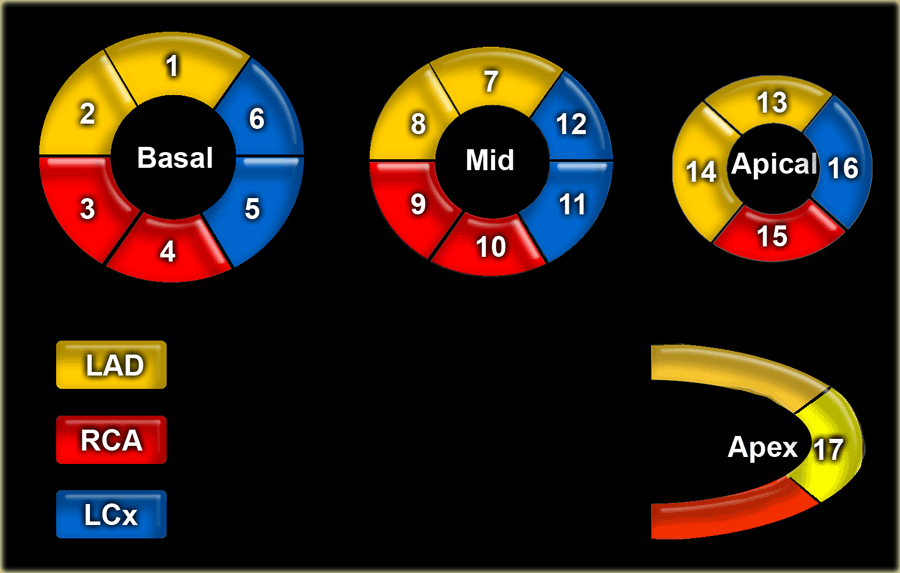
\includegraphics[width=0.5\linewidth]{./images/17_supply.png}
	\caption{Schematic representation of the supply to each segment (simplified).}
	\label{fig:segment_supply}
\end{figure}

\begin{figure}[H]
	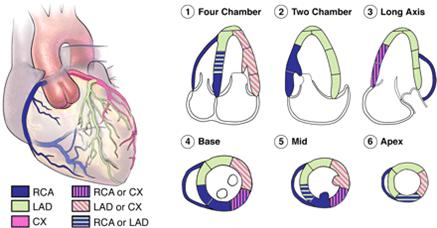
\includegraphics[width=0.5\linewidth]{./images/17_segment_2.jpg}
	\caption{Schematic representation of the supply to each segment.}
	\label{fig:segment_supply2}
\end{figure}

\subsection{Simulate myocardial perfusion}
\begin{table} [H]
\caption{Function requirements for function: Simulate myocardial perfusion}
\label{tab:funcsim}
This table specifies the requirements specific for the phantom that simulates the myocardial perfusion.
\begin{tabular}{l|p{120mm}|}
	\makecell[l]{\textbf{Requirement} \\  \textbf{number}} & \multicolumn{1}{c}{\textbf{Description}}\\
	\hline
	\sout{TFR-SIMT01} & \sout{An \ac{AIF} must be extractable from the left ventricle, as per software requirement.}\\
	TFR-SIM02 & Stenotic arteries are mimicked in a physiological way by physically narrowing (or increasing flow resistance) of certain arteries. \\
	TFR-SIMT03 & Different stenotic severity, should be possible by, for example, variable flow resistors or interchanging components. \\
	TFR-SIMT04 & The phantom must be compatible with D-SPECT protocol. \\
	\hspace{1.5cm} A) & Flow to the myocardium is supplied by the RCA, LAD, and LCx. \\
	\hspace{1.5cm} B) & Flow for each segment is supplied individually by branches of the RCA, LAD, and LCx, see figure \ref{fig:segment_supply}. \\
	\hspace{1.5cm} C) & Flow from each segment is measured separately such that they can be compared to the 17-segment model. \\
	\hspace{1.5cm} D) & An ROI for the AIF can be taken in the left atrium. Alternatively, the ROI for the AIF can be taken in the left ventricle. \\
	\hspace{1.5cm} \sout{E)} & \sout{An AIF can be taken from the left atrium.} \\
	\hspace{1.5cm} F) & The left ventricle's myocardium has a Vertical and Horizontal Longitudinal Axial (VLA/HLA) cross-sectional shape of a horseshoe. \\
	\hspace{1.5cm} G) & The left ventricle's myocardium has a Short Axial (SA) cross-sectional shape of a circle. \\
	TFR-SIMT05* & Phantom's compartment model should match the currently practised protocol.\\
	\hspace{1.5cm} A) & The contrast agent specified as Technetium (\textsuperscript{99m}Tc) tetrofosmin, see section \ref{sec:inj_contrast}. \\
	\hspace{1.5cm} B) & The contrast agent is absorbed by the myocardium to approximately 1.2\% of administered activity in 5 minutes. \\
	\hspace{1.5cm} C) & Contrast accumulates in skeletal muscles, spleen, liver, and kidneys (potential interference). \\
	\cline{2-2}
\end{tabular}
\raggedright
\textit{* \url{https://pubchem.ncbi.nlm.nih.gov/compound/131704316\#section=Absorption-Distribution-and-Excretion}}
\end{table}

\textbf{TFR-SIMT02} is based on the assumption that the relation between arteries, especially when some are narrowed, is too complex to be modelled independently. Simply reducing the overall flow in the myocardium will not capture that relation. Each segment of the left ventricle is supplied by a different branch of the three coronary arteries. One narrowed branch will have an impact on \textit{all} other branches, which leads to \textbf{TFR-SIMT03}. The severity of the stenosis will impact the other branches differently.

\textbf{TFR-SIMT03} is based on the goal of the project; to validate the D-SPECT. As mentioned in section \ref{sec:concept_oper}, the relatively less expensive, less invasive (patient friendliness and dose reduction), faster and more accurate system makes it suitable for myocardial perfusion imaging. However, the quantitative nature of the dynamic scanning protocol requires validation since it has not yet been done. Furthermore, the learning, educational, and training purposes of the phantom study is desired by researchers, manufacturers, and medical personnel. This is somewhat extended by \textbf{TFR-SIMT05}. Protocols already exist within clinics and is therefore the best starting point for research and phantom development.

\subsection{Inject tracer}
\label{sec:inj_tracer}
The injection protocol is not part of the development of the phantom. However, there are certain requirements to be monitored:

\begin{table}[H]
\caption{Textual requirements for function: Inject tracer}
\label{tab:injtrac_text}
\begin{tabular}{p{25mm}|p{115mm}|}
	\textbf{Requirement number} & \multicolumn{1}{c}{\textbf{Description}} \\
	\hline
	TRF-ICT01 			& Tracer volume is variable. \\
	TRF-ICT02			& Tracer activity is variable, also see TRF-ICQ03. \\
	TRF-ICT03			& Tracer agent is variable. \\
	TRF-ICT04 			& Tracer injection is reproducible.\\
	TRF-ICT05 			& Tracer protocol should match the currently practised protocol. \\
	\hspace{1.5cm} A) 	& See TRF-ICQ01. \\
	\hspace{1.5cm} B) 	& Tracer is injected, as bolus, via infusion pump. \\
	\hspace{1.5cm} C) 	& A pre-bolus is to precede the main bolus. \\
	\cline{2-2}
\end{tabular}
\end{table}

\begin{table}[H]
\caption{Quantitative requirements for function: Inject tracer}
\label{tab:injtrac_quan}
\begin{tabular}{p{25mm}|p{65mm}ccp{20mm}|}
	\textbf{Requirement number} & \multicolumn{1}{c}{\textbf{Description}} & \multicolumn{1}{c}{ } & \multicolumn{1}{c}{\textbf{Value}} & \multicolumn{1}{c}{\textbf{Unit}} \\
	\hline
	TRF-ICQ01 	& Tracer to be used. 			& = 			& \multicolumn{2}{p{35mm}|}{Technetium (\textsuperscript{99m}Tc) Tetrofosmin} \\
	TRF-ICQ02 	& Pre-bolus activity.			& = 			& 37				& Mega Becquerel \\
	TRF-ICQ03*	& Typical main bolus activity. 	& > \spacing < 	& 500 \spacing 700 	& Mega Becquerel \\
	\cline{2-5}
\end{tabular} \\
\raggedright
\textit{* hefty patient tend to get higher activity injected, i.e. 700 MBq.}
\end{table}

\section{Physical requirements}
\rrow{Determine size of seating of D-SPECT}
\rrod{Determine weight limit of seating of D-SPECT}
\rrot{Must it be completely anatomical?}
\rrot{Adjust requirements if the phantom does not have to be anatomical.}
The following requirements state the physical aspects of the phantom and of the .

\begin{table}[H]
\caption{Physical requirements (textual)}
\label{tab:physrec_text}
\begin{tabular}{p{25mm}|p{115mm}|}
	\textbf{Requirement number} & \multicolumn{1}{c}{\textbf{Description}} \\
	\hline
	TR-PRT01 			& The phantom is to be placed inside the QRM TRX-116, see TR-PRQ01. \\
	TR-PRT02 			& The phantom must fit on the D-SPECT seating in the imaging area. \\
	TR-PRT03 			& The phantom must be anatomically shaped. \\
	\hspace{1.5cm} \sout{A)} 	& \sout{In correspondence with requirements TFR-SIMT04.} \\
	\hspace{1.5cm} B) 	& Four chambered phantom that correspond to left/right ventricle and left/right atrium. \\
	\hspace{1.5cm} C) 	& Segmented myocardium surrounds heart chambers. \\
	\hspace{1.5cm}\sout{D)}	& \sout{Three coronary arteries, RCA, LAD and LCx, supply the myocardium.} \\
	\hspace{1.5cm} E) 	& The coronary arteries run outside of the myocardium. \\
	\hspace{1.5cm} F) 	& The coronary veins run outside of the myocardium. \\
	TR-PRT04 			& The flow set-up is to remain horizontal (preventing additional flow resistance). \\
	TR-PRT05 			& The phantom cannot contain air bubbles. \\
	\cline{2-2}
\end{tabular}
\end{table}

\begin{table}[H]
\caption{Physical requirements (Quantitative)}
\label{tab:physrec_quan}
\begin{tabular}{p{25mm}|p{65mm}ccp{20mm}|}
	\textbf{Requirement number} & \multicolumn{1}{c}{\textbf{Description}} & \multicolumn{1}{c}{ } & \multicolumn{1}{c}{\textbf{Value}} & \multicolumn{1}{c}{\textbf{Unit}} \\
	\hline	
	TR-PRQ01 & Short Axial diameter.		 						& < 			& 100 							& Millimetre \\
	TR-PRQ02 & Weight on patient chair. 							& < 			& 171 							& Kilogram   \\
	TR-PRQ03 & Phantom's outer dimensions. 							& 				& 								& 			 \\
	\hspace{1.5cm} A) & Basal-Apical distance. 						& $\approx$ 	& 120 							& Millimetre \\
	\hspace{1.5cm} B) & Left-Right Lateral distance.				& $\approx$ 	& 80							& Millimetre \\
	\hspace{1.5cm} C) & Anterior-Posterior distance. 				& $\approx$ 	& 60							& Millimetre \\
	TR-PRQ04 & Left ventricle dimensions.							& 				& 								& 			 \\
	\hspace{1.5cm} A)* & Internal Apical-Annular distance.			& > \spacing < 	& \invchar 69.4 \spacing 105.8	& Millimetre \\
	\hspace{1.5cm} B) & Internal Septal-Lateral distance. 			& > \spacing <	& 38.2 \spacing 55.6			& Millimetre \\
	\hspace{1.5cm} C) & Internal Anterior-Inferior.					& > \spacing < 	& 46.9 \spacing 68.5 			& Millimetre \\
	\hspace{1.5cm} D) & Myocardial wall thickness.					& > \spacing < 	& 4.8 \spacing 9.8				& Millimetre \\
	\hspace{1.5cm} E) & Internal volume.							& > \spacing < 	& \invchar 52.6 \spacing 143.6 	& Millilitre \\
	TR-PRQ05 & Right ventricle dimensions.							& 				&								&			 \\
	\hspace{1.5cm} A) & Internal Apical-Annular distance.			& > \spacing <	& 44.8 \spacing 79.2 			& Millimetre \\
	\hspace{1.5cm} B) & Internal Septal-Medial	distance.			& > \spacing < 	& 19.2 \spacing 40.0 			& Millimetre \\
	\hspace{1.5cm} C) & Internal Anterior-Inferior distance.		& > \spacing < 	& 42.2 \spacing 73.6 			& Millimetre \\
	\hspace{1.5cm} D) & Myocardial wall thickness.					& > \spacing <	& 1.0 \spacing 3.8				& Millimetre \\
	\hspace{1.5cm} E) & Internal volume. 							& > \spacing <	& \invchar 24.9 \spacing 139.3 	& Millilitre \\
	\cline{2-5}
\end{tabular} \\
\raggedright
\textit{* Annular $\rightarrow$ Annulus $\rightarrow$ assuming mitral valve level. }
\end{table}

\begin{table} [H]
\caption{Physical requirements}
\label{tab:physrec}
This table summarises the physical requirements.
\begin{tabular}{l|p{120mm}|}
	\makecell[l]{\textbf{Requirement} \\ \textbf{number}} & \multicolumn{1}{c}{\textbf{Description}}\\
	\hline

	TR-PR03 & The phantom must be placed inside a thorax phantom, QRM TRX-116, with maximum diameter of 100mm. \\
	TR-PR04 & Total weight, on patient chair, cannot exceed 171kg. \\
	TR-PR06* & The phantom must match the size of an average human heart, 12x8x6cm [LxWxD] \citep{openstax2013anatomy}. \\
	TR-PR07 & The phantom must resemble the weight of an average human heart, 250-300g (female) or 300-350g (male) \citep{openstax2013anatomy}. \\
	TR-PR08+ & The phantom's ventricles must match the volume of average human ventricles, between 40 and 180mL. \\
	TR-PR09+ & The phantom's atria must match the volume of average human atria, between 80 and 115mL. \\
	TR-PR10** & The phantom's ventricles must match the dimensions of an average human heart, between 60-90x30-50x60-90mm [LxWxD] \\
	\cline{2-2}
\end{tabular}
\raggedright
\textit{*Length (L): longitudinal axis (apex-basal), width (W): transverse axis (septal - lateral), Depth (D):  transverse axis (anterior-inferior).} \\
\textit{**Length (L): longitudinal axis (apical-annular), width (W): transverse axis (septal-lateral (LV) or septal-medial (RV)), depth (D): transverse axis (apical-annular)} \\
\textit{+\cite{chiribiri2013perfusion} uses LA/RA of 105mL and LV/RV of 120mL.}
\end{table}

\section{Environmental requirements}
\rrot{Determine how much noise output it may have.}
\rrod{Determine the height of the chair of the D-SPECT}
In what environment is the system operating.
\begin{table} [H]
\caption{Environmental requirements}
\label{tab:envirreq}
This table summarises the environmental requirements, i.e. the restrictions set by the environment to the phantom.
\begin{tabular}{l|p{120mm}|}
	\makecell[l]{\textbf{Requirement} \\ \textbf{number}} & \multicolumn{1}{c}{\textbf{Description}}\\
	\hline
	TR-ER01* &  No high-density or "High-Z" material is to be used.\\ 
	TR-ER02 & The phantom's left and front side must remain free such that the D-SPECT camera image around it. \\ 
	TR-ER03** & Any part of the flow set-up and/or phantom, that does not fit directly on the patient chair, must remain horizontal with the remaining parts between 63 and 93cm. \\
	\cline{2-2}
\end{tabular}
\raggedright
\textit{* High-density and "High-Z" material, i.e. material with high atomic number, tend to block gamma radiation emitted by \ac{SPECT} tracers. Examples are Titanium (Ti), Chromium (Cr), Vanadium (V), Iron (Fe), or Lead (Pb); atom number \textgreater 22, Lead is 82.} \\
\textit{** The patient chair's seating is adjustable between 63 and 93cm.}
\end{table}

\section{External interfaces}
\begin{table} [H]
\caption{External interface requirements}
\label{tab:exint}
This table summarises the requirements for the external interface.
\begin{tabular}{l|p{120mm}|}
	\makecell[l]{\textbf{Requirement} \\ \textbf{number}} & \multicolumn{1}{c}{\textbf{Description}}\\
	\hline
	TR-EI01 &  Live plotting, at 10Hz, of system system flow and pressure.\\
	TR-EI02 & Ability to adjust the output of the flow generators. \\
	TR-EI03 & Serial communication between control/monitoring systems and external interface.\\
	\cline{2-2}
\end{tabular}
\end{table}

\section{System qualities}
\rrot{Specify pressure threshold.}
Define the quality of the system: such as reliability, availability, serviceability, security, scalability, maintainability.
\begin{table} [H]
\caption{System qualities}
\label{tab:sysqual}
This table summarises the system qualities.
\begin{tabular}{l|p{120mm}|}
	\makecell[l]{\textbf{Requirement} \\ \textbf{number}} & \multicolumn{1}{c}{\textbf{Description}}\\
	\hline
	TR-SQ01 & The flow set-up must perform an emergency shut down when the arterial pressure exceeds specified threshold. \\ 
	TR-SQ2 & The flow set-up must perform an emergency shut down when the flow cannot be controlled, i.e. erratic. \\
	\cline{2-2}
\end{tabular}
\end{table}

\section{Constraints and Assumptions}
Design constraints that have been imposed and assumptions that have been made by the requirements engineering team when gathering and analyzijng the requirements.

\begin{table}[H]
\caption{}
\label{tab:constassump}
This table summarises constraints placed on the design and assumptions made to yield the system requirements.
\begin{tabular}{l|p{120mm}|}
	\makecell[l]{\textbf{Reference} \\ \textbf{number}} & \multicolumn{1}{c}{\textbf{Description}}\\
	\hline
	TR-CA01 &  Cardiac artefacts, beating of the heart, is initially too complex. The phantom will be static. \\
	TR-CA02 & Breathing artefacts are not simulated in the phantom itself. A breathing thorax phantom can be used if available. \\
	TR-CA03 & Chest size, the amount of tissue between heart and scanner, is not simulated in the phantom itself. Thorax phantoms with modular rings are available to simulate tissue patients with varying BMIs. \\
	\cline{2-2}
\end{tabular}
\end{table}
